\documentclass [titlepage,12pt,letter] {article}
\pagestyle{myheadings}

 
\usepackage{graphicx} 
\usepackage{epsfig}
\usepackage{subfigure}
\usepackage{fancyhdr}
\usepackage{url} 
\pagestyle{fancy}


\fancyhead{}
\fancyfoot{}
			
\lhead{CSC349A Lecture Notes}
\rhead{Little, Rich, George Tzanetakis}


\setcounter{page}{1}
\cfoot{\thepage}




\begin{document} 


These are the lecture notes for CSC349A Numerical Analysis prepared by
Rich Little and George Tzanetakis. They roughly correspond to
the material covered in each lecture in the classroom but the actual
classroom presentation might deviate significantly from them depending
on the flow of the course delivery. They are provided as a reference to
the instructor as well as supporting material for students who miss
the lectures. They are simply notes to support the lecture so the text
is not detailed and they are not thoroughly checked. Use at your own
risk.

\section{Course Logistics} 

Throughout the course I will try to give examples of how
ideas from Numerical Analysis are used in all sorts of cool
applications as well as how errors in the usage of Numerical Analysis
algorithms have had significant cost. 

I am going to experiment with using the graphics tablet in conjunction with the blackboard this term.

The use of the textbook is optional but it will
definitely help you understand deeper the material. Older editions are ok. 

I will NOT be recording the lectures or posting lecture recordings from previous classes.

The course outline can be found at:

\url{https://heat.csc.uvic.ca/coview/course/2023091/CSC349A} 

The course outline has an overview of the material that will be
covered and a rough schedule for the assignments and exams. 
There will be 5 to 10 assignments (worth a total of $30\%$ of the final
grade), two midterms worth $30\%$, and a final exam worth $40\%$. In
addition to the book handouts with notes about the various topics
covered will be provided online at the course webpage. A course pack
containing the course handouts is available on demand at the UVic
bookstore. Finally lecture notes such as this document will be
provided for most of the lectures. These notes are by no means a
substitute for attending the lectures and the material presented in a
lecture might deviate from what is on the notes.





\section{Importance of Numerical Analysis} 

A common view of Numerical Analysis is that it is boring, uninviting
field mainly concerned with the study of various types of errors. I
certainly felt that way when I took it for the first time as an
undergraduate. Over time my view of Numerical Analysis has
significantly changed and I have found that the ideas and concepts
learned in this course are used in a large variety of different
contexts and form the foundation of a lot of the software that we use
daily. One of my goals for this course is to convey this importance 
of Numerical Analysis in addition to covering the actual methods
themselves. 

Although the analysis of errors is central to Numerical Analysis it is
much more than that. Numerical analysis is the study of algorithms for
the problems of continuous mathematics.
``Continuous'' means that real or complex numbers are involved.
Because continuous numbers cannot be represented exactly on computers
errors are inevitable but need to be controlled.  ``Continuous''
problems are everywhere in Engineering and Computer Science including many areas that
you probably never thought had any connection with Numerical Analysis.

There is an incredible number of applications of numerial methods in
all fields of engineering and computer science. In many cases even
practitioners familiar with the application might not realize that
``under the hood'' of their techniques lie numerical analysis
methods. Throughout the course I will try to highlight some of these
applications and draw connections between what we are learning and
actual application areas. It is also interesting to look at the times
when misunderstandings or errors in numerical simulations have
resulted in enormous financial and in some ways human cost. Some 
examples of errors in numerical analysis can be found in the following
link: \url{http://www.ima.umn.edu/~arnold/disasters/disasters.html}. 

Here is a quick list of applications in which numerical methods play a
fundamental role. It is by no means exhaustive and it is a mixture of
more obvious applications and some that you probably never expected.
The first applications of computers were in the military. They include
discrete types of operations used in code breaking \footnote{\url{http://en.wikipedia.org/wiki/AlanTuring}} as well as continuous
mathematics in things like the computation of ballistic tables. The
origins of numerical methods lie in large scale computer simulations
initially for atomic bombs and later for things like climate modeling
but as computers became increasing smaller, faster and cheaper they
have expanded to all sorts of areas. Many computer games rely on
simulations of physics to create realistic experiences. Angry birds is
a popular example of how ballistics and Newtonian physics of motion
can be used to hit structures using angry birds. Animators
can use tools to model limbs, muscles individually but when it comes
to large number of objects interacting such as hair, water molecules
or Orcs in the Lord of the Rings movies physics simulation typically
using differential equations is utilized. Machine learning and data
mining is used in all sorts of application areas such as face
recognition, credit card ratings, hedge funds, business analytics and
the list goes on. Many modern machine learning methods (for example
support vector machines, neural networks, self-organizing maps) are
based on optimization methods.  Search engines exploit the structure
of links between web page and use methods from numeric analysis such
as singular value decomposition to analyze large graphs represented as
matrices. Computer networks, image processing, digital signal
processing, climate modeling all make heavy use of numerical
methods. In fact any time a computer program utilizes floating point
numbers for some computation it is using results from numerical
methods.

Basically numerical analysis algorithms are under everything. However
they tend to be rather invisible and hidden under layers of software
complexity. Software libraries such as {\it Lapack} and {\it BLAS}
are parts of all sorts of existing software packages that are built on
top of them. A lot of this code was originally written in Fortran and
although the number of programmers who write in Fortran is diminishing
they are still kept around as they work well and are so widely
used that to some extent Fortran compilers are simply kept around to
keep these libraries and software packages going. Even if you never
``use'' directly this library chances are you have used some software
that does and getting some glimpse of what they do which you will in
this course is a great way to appreciate the complexity and
interdependency of software. 


\section{Book Overview} 

The book has 8 parts and 32 chapters. Each parts begins with a Preface
that has the motivation behind the problems covered and some
background mathematics for that particular part. 


Numerical Analysis is important in Science and Engineering. 

\begin{itemize} 
\item{It provides powerful problem solving tools that can handle large
     amounts of data, non-linearities, and complex geometries (such
     problems can not be solved by any other means).}
\item{Intelligent use of packaged software often requires knowledge of
    the basic underlying theory} 
\item{Package software cannot solve all real-world problems (you may
    have to design your own programs).} 
\end{itemize} 

The following major topics will be covered in each part: 

\begin{itemize} 

\item{Part 1: Modelling, Computers and Error Analysis}
\item{Part 2: Roots of equations. Solve $f(x) = 0$ for $x$.}
\item{Part 3: Linear algebraic equations:. Given the $a$'s and the
    $b$'s solve 
\begin{eqnarray}
a_{11}x_{1} + a_{12} x_{2} = c_{1} \\ 
a_{21}x_{1} + a_{22} x_{2} = c_{2} 
\end{eqnarray} 
\noindent 
for the $x$'s. }
\item{Part 5: Curve Fitting: Regression or Interpolation}
\item{Part 6: Integration: $I = \int_{a}^{b} f(x) dx$ Find the area
    under the curve.}
\item{Part 7: Ordinary differential equations: Given $\frac{dy}{dx}=f(x,y)$ solve for $y$ as a function of $x$.}
\end{itemize} 


\section{A Motivating Example} 

Determine the terminal veloctiy of free-falling body (a parachutist)
near the eart's surface. Mathematical Model: Newton's second law of motion: 

\begin{equation} 
F = m a 
\end{equation}  
\noindent 
where $F$ is the force (measured in Newtons), $m$ is the mass
(measured in kg), and $a$ is the acceleration (measured in $m/s^2$). 
Acceleration is by definition the time rate of change of the
velocity: 
\begin{equation} 
a = \frac{F}{m} 
\end{equation} 

Now consider a free falling object (a parachutist or an angry
bird). There are two forces that operate on this object: the downward
pull of gravity ($F_{D})$ and the upward force of air resistance ($F_{U}$). 

\begin{equation} 
F = F_{D} + F_{U}
\end{equation} 


These equations are typical of mathematical models of the physical
world: 

\begin{itemize} 
\item{Describes a natural process in mathematical terms}
\item{It represents an idealization and simplification of reality} 
\item{It yields reproducible results and can be used for predictive
    purposes} 
\end{itemize} 


\begin{equation} 
F_{D} = m g 
\end{equation} 

\noindent 
where $m$ is the mass and $g$ is the acceleration due to gravity 
which is approximately equal to $9.8\;\;m/s^2$. We will assume a
simple model of air resistance in which it is linearly proportional to
velocity and acts in an upward direction i.e: 

\begin{equation} 
F_{U} = - c v
\end{equation} 

\noindent where $c$ is the drag coefficient (a constant that accounts
for the properties of the falling object such as as shape, type of
surface etc). 
Therefore the net force is: 

\begin{equation} 
F = m g - c v
\end{equation} 

\noindent and by using the fact that the acceleration is the
derivative of the velocity we can derive the following mathematical
model: 

\begin{equation} 
\frac{dv}{dt} = g - \frac{cv}{m} 
\end{equation} 

\noindent 
This is a differential equation that relates the acceleration of a
falling object to the forces acting on it. It is possible to get an
analytic solution to this differential equation using calculus. If the 
object is initially at rest i.e $v = 0$ at time $t = 0$ then: 

\begin{equation} 
v(t) = \frac{gm}{c} (1 - e^{-\frac{ct}{m}})
\end{equation} 


This analytical solution can be used directly to solve
problems. \footnote{For those of you who are interested it is
  straightforward to show that the analytical solution satisfies the
  differential equation by substituting in the left hand side and
  differentiating and substituting in the right hand side. After a few
straightforward algebraic manipulations you can show the two sides are
equal. To derive the analytical solution you need to express the
derivative and then take the limit of the resulting series.} 


For
example a parachutist of mass $68.1 kg$ jumps out of a stationary hot
air balloon. The drag coefficient is equal to $12.5 kg/sec$. 

Inserting the parameters into the equation we get: 

\begin{equation} 
v(t) = \frac{9.81 (68.1)}{12.5} (1 - e^{-(12.5/68.1)t}) 
\end{equation} 

\noindent 
this equation can be used directly to compute the various values of
velocity for different values of $t$. For example: 

\begin{table}
\centering
\begin{tabular}{|c|c|} 
\hline
{\bf t}    & {\bf v} \\ 
\hline 
0   &  0.0 \\ 
2   &  16.40 \\ 
4   &  27.77 \\ 
6   &  35.68  \\
..   &  ..  \\
$\infty$ & 53.44 \\  
\hline
\end{tabular}
\end{table} 
  

After a sufficiently long time a constant velocity, called {\it
  terminal} velocity of $53.44 m/sec$ is reached as eventually 
the air resistance which keeps increasing as the velocity increases
will become equal with the force of gravity which remains constant. 

Another possibility is to try to use a numercial (in constrast to an
analytical approach) for solving this mathematical model. Even though
our solution will not be exactly the same depending on how much
accurate we want to be we can make it arbitrarily close. There are
several reasons to do so: 
\begin{itemize} 
\item{Numerical methods can be applied to functions for which we can
    not easily find an analytical solution through Calculus} 
\item{As any equations is to some degree an approximation of reality
    and therefore errors are inevitable it is possible depending on
    the application that the errors introduced by the numeric
    approximation are neglible in the context of the desired
    application} 
\item{It's extremely simple to write a computer program to do the job 
for us although the number of mathematical operations involved is much
larger than the analytical solution} 
\end{itemize} 

The idea is rather simple. We will approximate the derivative of the
function by a ``finite divided difference'' effectively discretizing
time. If we denote the discrete time steps we take as $t_{i}$ (we can decide what 
sampling rate is appropriate depending on the application) then we can
approximate the derivative at time $t_{i}$ as follows: 

\begin{equation} 
\frac{dv}{dt}(t_{i}) \approx \frac{\Delta v(t)}{\Delta t} = \frac{v(t_{i+1}) - v(t_{i})}{t_{i+1} - t_{i}}
\end{equation} 

We can substitute this equation into our parachutist model to give: 

\begin{equation} 
\frac{v(t_{i+1}) - v(t_{i})}{t_{i+1} - t_{i}} \approx g - \frac{c}{m} v(t_{i})
\end{equation} 
\noindent 
this can be rearranged to yield: 
\begin{equation} 
v(t_{i+1}) \approx v(t_{i}) + (g - \frac{c}{m}v(t_{i}))(t_{i+1} - t_{i})
\end{equation} 

Notice that this equation gives us a way to compute the velocity value
at time $t_{i+1}$ based on the previous value of the velocity. This
approach is called Euler's method can be verbally expressed as: 
{\it New value = old value + slope x step size}. For example we can
use it to compute the velocity values with a step size of $2$
seconds. 

At the start of the computation we use an initial velocity value
$v_{0} = 0$ for $t_{0} = 0$ plug the numbers into the equation 
and get the value of $v_{1}$. Then we can use the value at $v_{1}$ to 
compute the value at $v_{2}$ and so forth. 


\begin{table} 
\centering
\begin{tabular}{|c|c|} 
\hline
{\bf t}    & {\bf v} \\ 
\hline 
0   &  0.0 \\ 
2   &  19.62 \\ 
4   &  32.04 \\ 
6   &  39.90  \\
..   &  ..  \\
$\infty$ & 53.44 \\ 
\hline
\end{tabular}
\end{table} 


\begin{figure}[ht]
  \centering
  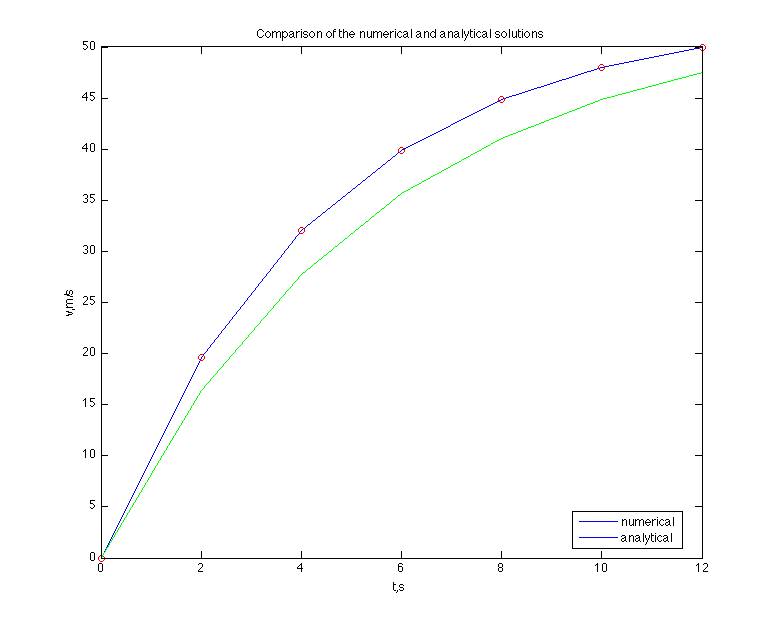
\includegraphics[scale=0.5]{comparison_numerical_analytical}
  \caption{Comparison of numerical and analytical solution}
  \label{fig:comparison}
\end{figure}





\noindent 

Figure ~\ref{fig:comparison} shows a plot comparing the results of the
numerical approximation using Euler's method and the exact analytical
solution. In engineering there is frequently a tradeoff between
accuracy and computational resources. 
The Euler method and more
generally numerical methods allow you to control that tradeoff for
example by adjusting the step size appropriately for the program at
hand. There are several questions one could ask at this point that we
will be exploring in the rest of the course. For example can we show
that the error between the exact solution and the numerical
approximate solution will always decrease with smaller step size ? Can
we compare how long different approaches to approximating the
derivative of a function take ? Are there any functions for which this
would not work ? Could we reduce the number of
multiplication/additions needed to perform each step of the iteration
?

\section{Reading and Further Reading} 

The material covered in this lecture corresponds to Chapter 1 of the
textbook. The article ``The Definition of Numerical Analysis'' by
Lloyd N. Trefethen makes a good case for Numerical Analysis being a
far more interesting field that simply the study of errors and defines
it as the study of algorithms for continuous mathematics. 

I also mentioned Alan Turing whose efforts during World War II 
to break the codes used by the Germans led to the development 
of electronic computers. The Wikipedia article on him 
is thorough and definitely worth reading: 
{\url http://en.wikipedia.org/wiki/Alan_Turing}. 

\bibliographystyle{IEEEbib} 
\bibliography{csc349a} 

\end{document} 











